\documentclass[9pt,twocolumn,twoside]{pnas-new}
% Use the lineno option to display guide line numbers if required.
% Note that the use of elements such as single-column equations
% may affect the guide line number alignment. 

\templatetype{pnasresearcharticle} % Choose template 
% {pnasresearcharticle} = Template for a two-column research article
% {pnasmathematics} = Template for a one-column mathematics article
% {pnasinvited} = Template for a PNAS invited submission

\usepackage{amsthm}
\usepackage{amsmath}
\usepackage{amssymb}

\DeclareMathOperator*{\argmax}{argmax}
\newtheorem{corollary}{Corollary}
\newtheorem{axiom}{Axiom}
\newtheorem{theorem}{Theorem}
\newtheorem{definition}{Definition}
\newtheorem{lemma}[theorem]{Lemma}

\title{A way around the exploration-exploitation dilemma.}

% Use letters for affiliations, numbers to show equal authorship (if applicable) and to indicate the corresponding author
\author[a,1]{Erik J Peterson}
\author[a,b]{Tim Verstynen}
\affil[a]{Department of Psychology}
\affil[b]{Center for the Neural Basis of Cognition, Carnegie Mellon University, Pittsburgh PA}

% Please give the surname of the lead author for the running footer
\leadauthor{Peterson} 

% Please add here a significance statement to explain the relevance of your work
% \significancestatement{TODO}

% Please include corresponding author, author contribution and author declaration information
% \authorcontributions{EJP?.}
\authordeclaration{The authors have no conflicts of interest to declare.}
% \equalauthors{\textsuperscript{1}A.O.(Author One) and A.T. (Author Two) contributed equally to this work (remove if not applicable).}
\correspondingauthor{\textsuperscript{1}To whom correspondence should be addressed. E-mail: Erik.Exists@gmail.com}

% Keywords are not mandatory, but authors are strongly encouraged to provide them. If provided, please include two to five keywords, separated by the pipe symbol, e.g:
% \keywords{Keyword 1 $|$ Keyword 2 $|$ Keyword 3 $|$ ...} 

\begin{abstract}
The exploration-exploitation dilemma is considered a fundamental problem in the learning and decision sciences. Exploitation means choosing the best known option. Exploration means searching among unknown options to find one more valuable than the present best. Some searches may be brief and successful. Other long and unsuccessful. It's impossible to know which until the search is complete. This uncertainty, often referred to as partial observability, makes the problem of exploration mathematically intractable. Focusing only on rewards though ignores the direct and certain value of exploratory behavior: the acquisition of information about the world. Here, we challenge the traditional approach to the dilemma and offer an alternative account based in information theory. We first derive an axiomatic measure of information value. We use this to decompose the exploration-exploitation dilemma into a tractable two-part problem, creating separate mathematical objectives for exploration and exploitation. From this we derive a new meta-policy approach which optimally maximizes total information value and maximizes total rewards. In simulation, we show how this policy generates useful and naturalistic behavior in both simple and complex simulated worlds. 

% Finally we who how this same theory predicts exploratory actions of \textit{EVERY FUCKING LIVING THING?!}. % TODO....
\end{abstract}

% \dates{This manuscript was compiled on \today}
% \doi{\url{www.pnas.org/cgi/doi/10.1073/pnas.XXXXXXXXXX}}

\begin{document}
\verticaladjustment{-2pt}
\maketitle

\thispagestyle{firststyle}
\ifthenelse{\boolean{shortarticle}}{\ifthenelse{\boolean{singlecolumn}}{\abscontentformatted}{\abscontent}}{}
Animals across the animal kingdom will a new environment even when no rewards, like food and water, are present or expected. Many of these same animals also explore as play, trying to understand other agents behavior, to the learn the best playful strategies, and to refine their action repertoires. Of course animals like bees, mice, monkey, and humans also explore to find more rewards. In a general sense then it seems animals explore to gain information \textit{and} to acquire more rewards. These two goals are often conflated during reinforcement learning.

When an animal explores looking for rewards there is a trade-off to be made between with choosing more conservative actions, likely to produce desirable results (what we call exploitation), and exploring to try are beat the current best option. The optimal policy for exploitation is well known. One calculates total expected future rewards. The optimal policy for exploration, on the other theoretical hand, remains elusive \citep{thrun1992active, dayan1996exploration, findling2018computational, gershman2018deconstructing}. 

Exploration is often costly, which makes it hard to theoretically explain using rewards. To mitigate this ``cost'', exploration is often reframed as a problem of ``information seeking'' and fictive rewards are introduced. Fictive rewards can implemented as novelty or other motivational bonuses \citep{Sutton1990, dayan1996exploration}, or modeled as the internally generated isomorphism of tangible external rewards (so-called intrinsic rewards).  

Rebalancing reward with information seems simple and intuitive, but it comes with a fundamental limitation. If the goal is to maximize $r$, as defined by the dilemma problem, adding a fictive reward obscures this actual aim. After all, an increase in $V$ can come from a $r$ or from the fictive $\beta I$. Fictive rewards may encourage exploration but still offer no guarantee of a performance increase in the long term, once the fictive signal fades.

Here we propose \textit{information is valuable for its own sake}. We separate the two goals into two objectives. In our view agents should seek to maximize information value just as vigorously as reward. Their policies for reward learning should be separated from their policies for exploration. 

Our contributions are threefold. We first set out a series of axioms to serve as principled basis for information value, and use these to implement a working scheme rooted in information theory. Next we develop an optimal policy for exploration that maximizes information value. This theory is purely deterministic, meaning exploration no longer relies on random sampling and is instead perfectly rational. Finally, we derive a new \textit{meta-policy} which allows for simultaneously optimal and deterministic solutions to \textit{both} the problems of exploration and exploitation.

\section*{Results}
The overall objective in reinforcement learning is to maximize $V^{*}_{pi_R}$, expectation of total future rewards (Eq~\ref{eq:total_r}; \cite{Sutton2018}). When a fictive reward signal is present, this becomes Eq~\ref{eq:total_r_I}.

\begin{equation}
    V^{*}_{\pi_R} = \sum_{t \in T, s \in S} r
    \label{eq:total_r}
\end{equation}

\begin{equation}
    V^{*}_{\pi_R} = \sum_{t \in T, s \in S} r + \beta I
    \label{eq:total_r_I}
\end{equation}

Where $I$ is a generic stand in for the pack of fictive possibilities--including novelty bonuses, curiosity signals, or entropy terms--and rewards are denoted by $r$, with $\beta$ is used for the fictive weight. For convenience, we confine rewards to be a binary variables, and $I$ to the real numbers ($r \in \{0, 1\}, I \in \mathbb{R}, \beta > 0$).

We propose that reinforcement learning should often become a two objective problem, maximizing both Eq.~\ref{eq:total_r_2} and Eq.~\ref{eq:total_e}. 

\begin{equation}
    V^{*}_{\pi_R} = \sum_{t \in T, s \in S} r
    \label{eq:total_r_2}
\end{equation}

\begin{equation}
    V^{*}_{\pi_E} = \sum_{t \in T, s \in S} I
    \label{eq:total_e}
\end{equation}

As we'll see in coming sections using separate objective let's us offer theoretical guarantees for exploration quality, rooted in dynamic programming. It also means we can motivate exploration without obscuring the ability to optimize rewards. Assuming the learning about the environment is possible, the net result is we can guarantee an optimal rewarding policy is found.

\subsection*{Information is not a reward}
A first principle analysis of information and reward shows they have opposing properties:

\begin{enumerate}
    \item Rewards are a conserved resource. Information is not. 
    \item The same kind of reward can be consumed many times without necessarily losing value\footnote{In practice, there are satiety effects but these are not a necessary part of the reward's value}. Information once learned has no value in being be learned again.
\end{enumerate}

These can be seen more intuitively by example. In \textit{1.}, If a rat shares its potato chip with a cage-mate, it has less food for itself. Compare that chip to a new idea. Explaining a new idea to lab-mate does not require forgetting the idea yourself. In fact, it's often the opposite.

In \textit{2.}, eating one potato chip often means wanting another. Where as if you know the capital of the United States, there is no value in being told the capital of the United States is Washington DC.

These philosophical differences lead to notable mathematical differences. To evenly share a reward $r$ between $n$ others, $r_n = \frac{r}{n}$. Where as for information value can in principle be shared without loss, so $I_n = I$. Likewise, if an animal is learning about some state of world $s$ the value of information about $s$ should decrease with time. Assuming learning can asymptote, then as $t \rightarrow \infty, I_s \rightarrow 0$. For rewards, value never changes. So as $t \rightarrow \infty, r_s \rightarrow r_s$.\footnote{Though including reward satiety effects may somewhat diminish $r_s$ in practice.}

For empirical, philosophical, and mathematical reasons we've suggested reward and information should be optimized separately. To make this suggestion formal in the next sections we \textit{1.} derive a general measure information value using an axiomatic approach, \textit{2.} derive a deterministic optimal policy to maximize this measure, and \textit{3.} derive a new optimal learning rule which can simultaneously maximize information \textit{and} reward value. We also show how efficient coding can lead to efficient re-exploration in environments that change with time. 

    
% ---------------------------------------------------------------------------
\subsubsection*{If information is not a reward, how can we value it}
Shannon originally developed information theory without any sense of what information ``means''. He focused on simply transmitting symbols. To work the theory does need to know what those symbols refer to, and is therefore extremely general \citep{Shannon1948}. Many attempts have since been made to instill information theory with meaning \citep{Kolchinsky2018}, and with meaning value follows. Most of these attempts require a ``salience'', or ``relevance'', or ``training'' signal (where all three terms amount to near the same thing), while others have taken an evolutionary approach \citep{Kolchinsky2018}.  
% TODO bump up refs

Instead of trying to define meaning more broadly, we take an axiomatic approach to define value: \textit{listing key properties (axioms) that any naturalistic measure of information value should have, and arrive a metric that satisfies these}. Put another way, we suggest information value can be strictly internal to an agent, but that meaning requires an explicit outside reference. This purely self-referential approach to information value is extremely general for the same reasons as Shannon's original theory. We only compare distributions, and do not consider what those distributions refer to.

We begin formalizing information value with four axioms:

\begin{axiom}
    The value of information about some event $x$ depends \textit{only} on what is already known about $x$ (and not $x$ itself).    
    \label{ax:1}
\end{axiom}
\begin{axiom}
    Information about some event $x$ that is known with no uncertain has a value of exactly 0.
    \label{ax:2}
\end{axiom}
\begin{axiom}
    The value of information about some event $x$ is non-negative. 
    \label{ax:3}
\end{axiom}
\begin{axiom}
    For a some set of events $X$, specific (or localized) changes to the local structure of the distribution $p(X)$ uncertainty are more valuable than global changes.
    \label{ax:4}
\end{axiom}

Axiom~\ref{ax:1} closes value calculations over the agent making them. Informally, we capture the idea that ``subjective value depends only on the subject's own experience''.  In Axiom~\ref{ax:2} we capture the idea that, ``if you know something \textit{perfectly}, there is no value in learning it again''. Axiom~\ref{ax:3} exists to impose that idea that, ``learning new information is always good, in principle''. In practice, of course, learning some new information can have undesirable consequences. But any these consequences are not part of the information itself, but live in its use. Axiom~\ref{ax:4} covers the precept that, ``specific information is more valuable than general information.'' 

To separate all fictive rewards from those which satisfy our axioms, we introduce a new term $E$ to represent axiomatic information value.

% ---------------------------------------------------------------------------
\subsubsection*{Using the KL divergence}
% TODO: https://twitter.com/simondedeo/status/993881889143447552?lang=en
% use the above tweet to show how KL is useful as info gain, in predicting attention, etc.

Calculations in information theory are done over probability distributions $p(.)$, on some set of symbols $S$. Here, symbols are states of the world (a notion we fully formalize below). 

\begin{definition}
    We call a distribution over a set of states $S$ a ``memory distribution'' and denote it with $M$, where $M(s) = p(s), \ \text{where} \ s \in S, \ p(.) \rightarrow (0, 1)$.
\end{definition}

The Kullback--Leibler divergence satisfies all four value axioms (Eq.~\ref{eq:KL}). 

\begin{equation}
    KL(M', M) = \sum_{s \in S} M'(s) \text{log} \frac{M'(x)}{M(x)} 
    \label{eq:KL}
\end{equation}

\begin{definition}
    Let $E$ represent value of information, such that $E = KL(M', M)$ (Eq.~\ref{eq:KL}), where $M$ is some initial memory and $M'$ is an update memory after observing some state $s'$.
\end{definition}

Axiom~\ref{ax:1} is satisfied by limiting $E$ calculations to successive memories. Axiom~\ref{ax:2}-\ref{ax:3} are naturally satisfied by KL. That is, $E = 0$ if and only if $M' = M$ and $E \geq 0$ for all pairs $(M, M')$.

To make Axiom~\ref{ax:4} more intuitive, in Figure~\ref{fig:metrics_specifity} we show how KL changes between an initial distribution (always shown in grey) and a ``learned'' distribution (colored). For simplicity's sake we use a simple discrete distribution, representing the likelihood of the first four non-negative integers $(0,1,2,3)$. Though the illustrated patterns should hold true for any pair of distributions. In Figure~\ref{fig:metrics_specifity} we see KL increases substantially more, for a the same local increase in probability, when that increase comes with a localized decrease, rather than with an even re-normalization (compare panels \textit{}{a.} and \textit{b.}).

\begin{figure}
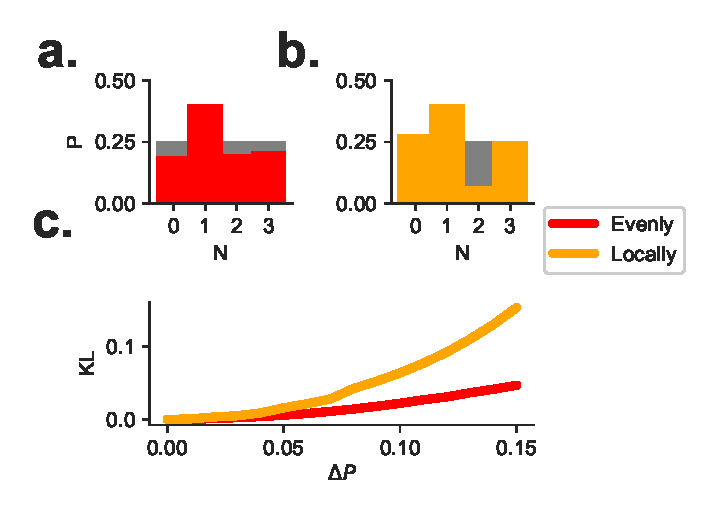
\includegraphics[width=0.4\textwidth]{figures/metrics_specifity.eps}
\caption{
\textit{Local probability structure and information value. Both distribution shown in a. and b. have the same total increase in the probability of a ``1'' appearing.
For \textbf{a.}  the necessary corresponding decrease in probabilities for all numbers (0, 2, 3) is evenly redistributed.
In \textbf{b.} the loss is focused locally on ``2''. 
\textbf{c.} The KL divergence increases more rapidly for local changes in probability density}}
\label{fig:metrics_specifity}
\end{figure}

% TODO: move this to the discussion?
To a skeptical reader Axiom~\ref{ax:4} may seem overly opinionated. A simpler natural set of Axioms is to keep 1-3 but replace~\ref{ax:4} with a new Axiom  that only requires information value track the total change in probability flux, that is $E \sim dP$. For this metric, the curves in Figure~\ref{fig:metrics_specifity} would overlap. We considered this, but felt this simpler view is incomplete. Information value should favor more specific, therefore more actionable, information. 

Given that KL measures the information gain (or loss) between two models, and has a long and useful history %TODO CITE
we could have skipped the Axiomatic approach and made a direct argument for KL. We did not do this for two reasons. 

First, the value of a reward is based on its biological significance via the law of effect. If were are to value information for its own sake we felt it was critical to base that value not on a particular theoretical view (i.e. information theory) but instead on a firm set the theory-independent principles. We felt obliged to first answer the question, ``if information is valuable, what do we base that value on?''. From this general point its much easier to make a practical implementation. 

Second, though (Shannon) information theory and KL are very useful constructs, they require symbolic and probabilistic representations. We don't know whether animals actually maintain such exact representations %\cite{TODO}. 
Likewise, in machine learning memory modules often don't rely on distributions, and instead simple recall selections of previous events %\cite{TODO}. 
The axioms can be easily satisfied in these alternative kinds of cases. A set of axioms also is a concrete point to debate how to value information; We hope ours isn't the last word.


% ---------------------------------------------------------------------------
\subsection*{Information value as a dynamic programming problem}
It is standard to embed the reinforcement learning problems into a Markov decision space. In this space, each state transition from $s_t$ to $s_{t+1}$ is independent of the history of transitions $S_{<t}$. Each transition generates a reward $r$, whose value is also independent of past states. Our definition of information value $E$ this formalism for $r$ as $E$ does dependent on past states through the memory $M$. However, $E$ is calculated iteratively over $M$ and a pair pf states $(s, s'$ and yields a non-negative real value with each iteration (i.e $E_{(s,s')} \ge 0, E \in \mathbb{R}^1$.  This simple sequential dependence leaves is consistent with dynamic programming formulation of the problem, which provide a route to discovering an optimal policy for maximizing the total information value. 

Introducing our formalism, we say at point in time $t$ an agent occupies a state $s$, and use $T$ to the final time horizon, which can be infinite, $T \leq \infty$. In practice a state $s$ may be a as simple as a position in space, the current visual input, or any other combination of sense information. To keep the theory tractable, we assume that the total number of states an animal might visit $S$ is finite. Formally then, $s\ in \textbf{S}; \textbf{S} \in \mathbb{R}^N$, where we use real numbers to represent states and $N$ is the total number of states. Again to keep analysis the analysis tractable we limit the number of actions $a$ animal might take to finite real set, $a \in \textbf{A}; \textbf{A} \in \mathbb{R}^K$, with $K$ actions. 

To take an action, we say an that animal consults its policy function, $\pi$. 

\begin{definition}
    Let $\pi$ be a policy function that maps a state $s$ to an action $a$, $\pi : s \rightarrow a$, such that $s \in S, a \in A$.
\end{definition}

State transitions are modeled with a transition function $\Lambda$ which combines the current state $s$ and an action $a$ to generate some new state $s'$.

\begin{definition}
    Let $\Lambda$ be a transition function which maps a $(s,a)$ 2-tuple to a new state $s'$, $\Lambda : (s, a) \rightarrow s'$.     
\end{definition}

A policy function and transition function combine to generate a path $P$. We use $t$ to index into $P$. 

\begin{definition}
    Let $P$ be a finite ordered collections of states $s$, such that $s \in S$ and the length of $P$ is $T$. We define $P$ recursively, $P(t+1) \leftarrow \Lambda(P(t), \pi_E(P(t)))$.
\end{definition}

Learned information is stored in a finite perfect (i.e., noiseless) memory $M$. 
    
\begin{definition}
    Let $M$ is probability distribution, over a set of $S$ and actions $A$, such that $M \in (0, 1)^{N\text{x}K}$. By independent we mean that the representation for any $s \in S$ and $a \in A$ can be updated without effecting the probabilities. 
\end{definition}

The independent representation of $S$ and $A$ probabilities is critical to all the optimality proofs presented here. Though in the natural world, the need for a well defined memory system is a clear requirement for nearly any learning system.

\begin{definition}
    Let $\mathcal{L}$ be a loss function that maps a memory $M$ and an state $s$, into an error term $\delta$. $L : s, M \rightarrow \delta$.
\end{definition}

\begin{definition}
    Let $U$ be an memory update function that maps a error $\delta$, a memory $M$ to a new memory $M'$, $U : s, \delta \rightarrow M'$.
\end{definition}

\begin{definition}
    Let $J$ be a learning rule that maps a memory $M$, a new state $s'$ into memory $M'$. That is, $J : M, s' \rightarrow M'$ subject to the constraints  $M' = U(s' \delta)$, $\delta = \mathcal{L}(M, s')$.
\end{definition}

\textit{With a loss of generality}, we assume that $\mathcal{L}$ is convex, and that every observation $s$ leads to learning progress, unless $L(s) = 0$. That is, the gradient of $\triangledown \mathcal{L} < 0$ for all $s \in P$ when $L(s) \neq 0$ and. The strong assumptions of convexity, and continual learning progress greatly simplifies the critical theorems for exploitation we prove, but is also overly restrictive. Having completed the initial proofs, we explore under what conditions these constraints can be safely relaxed.

We discuss our measure of information value $E$ in detail in the previous section, but for completeness we reintroduce it with complete formal notation.

\begin{definition}
    Let $E(s)$ be the information value between two successive memories, $M$ and $M'$. where $E(s) := KL(KL(M', M) = \sum_{s \in S} M'(s) \text{log} \frac{M'(s)}{M(s)} $. The new memory $M'$ follows from the state transition $s' \leftarrow \lambda (s, a)$ (which is in turn driven by the action policy $a = \pi(s)$), a loss calculation $\delta = \mathcal{L}(s, M)$, and the learning rule update $M' = J(M, \delta)$
\end{definition}

For consistency with dynamic programming and the Bellman equation, we make a change of notation for $E$ by introducing a payoff function $F$.

\begin{equation}
    \begin{split} \label{eq:V}
    F(M_t, a_t) = E(M_{t+1}, M_{t})\\
    \text{subject to the constraints} \\
    s_{t+1} = \Lambda(s_t, a_t),\\ 
    M_{t+1} = J(M_t, s_{t+1})
    \end{split} 
\end{equation}

The total information value is then simply the sum of all payout functions for some policy $\pi_E$ observation period $T$. 

\begin{equation} \label{eq:V}
    \begin{split}
        V_{\pi_E} = \sum_{t \in T} F(M_t, a_t)\\
        \text{subject to the constraint}\\
        \forall t = (0,1,2,\ldots, T),\ T \leq \infty
    \end{split}
\end{equation}

% --------------------------------------------------------------------------
\subsubsection*{A proof of optimal substructure}
A first step in solving a dynamic programming problem is isolating the relevant subproblem, and proving it has an optimal substructure. Which means the problem can be decomposed into an iteratively optimal series. This property in inherent in the Markov Space % TODO cite, 
but is not guaranteed in the more general space we need to work with in estimating the best was to maximize total information value. Information value and its payoff function $F$ depend on the memory $M$ and so need to prove learning progression on $M$ has an optimal substructure.

% TODO need to adapt for ties.... see coursera
\begin{theorem} \label{theorem:opt_sub}
    Assuming transition function $\Lambda$ is deterministic, if $V^*_{\pi_E}$ is the optimal information value given by $\pi_E$, a memory $M_t$ has optimal substructure if the the last observation $s_t$ can be removed from $M_t$, by $J^{-1}(M_t, s_t) \rightarrow M_{t-1}$, such that $V^*_{t-1} = V^*_t - F(M_t, a_t)$ is also optimal. 
\end{theorem}
\begin{proof}
    For the sake of contradiction, assume there exists an alternative policy $\hat \pi_E$ that gives a memory $\hat M_{t-1} \neq M_{t-1}$ and for which $\hat V^*_{t-1} > V^*_{t-1}$. 

    To recover the known optimal memory $M_t$ we lift $\hat M_{t-1}$ by $U(\hat M_{t-1}, s_t) \rightarrow M_t$, but this lifting implies $\hat V^* > V^*$, which contradicts the purported optimality of $V^*$ and therefore $\pi_E$.
\end{proof}


% --------------------------------------------------------------------------
\subsubsection*{An optimal recursive policy}
In terms of the payout $F$ and policy $\pi_E$ and some initial memory $M_0$ the optimal value is given by Eq~\ref{eq:V_star}.

\begin{equation} \label{eq:V_star}
    \begin{split}
        V^*_{\pi_E}(M_0) = \max_{\{a\}_{t \in T}} \sum_{t \in T} F(M_t, a_t)\\
        \text{subject to the constraint}\\
        \forall t = (0,1,2,\ldots, T),\ T \leq \infty
    \end{split}
\end{equation}

Knowing the memory $M$ has optimal substructure (Theorem~\ref{theorem:opt_sub}) the valuation of $V_{\pi_E^*}(s_0)$ can be decomposed into a series of local greedy decisions.

\begin{equation} \label{eq:bellman_seq}
    \begin{split}
        V^*_{\pi_E}(M_0) &= \max_{\{a\}_{t \in T}} \Big [\sum_{t \in T} F(M_t, a_t)\Big ]\\
                         &= \max_{\{a\}_{t \in T}} \Big [F(M_0, a_0) + \sum_{t \in T}F(M_{t+1}, a_{t+1})\Big ]\\
                         &= F(M_0, a_0) + \max_{\{a\}_{t \in T}} \Big [\sum_{t \in T} F(M_{t+1}, a_{t+1}) \Big ]\\
                         &= F(M_0, a_0) + V^*_{\pi_E}(M_{t+1}) + V^*_{\pi_E}(M_{t+2}),\ \ldots
    \end{split}
\end{equation}

From the final entry in Eq.~\ref{eq:bellman_seq}, we can write down an optimal recursive definition for $V^*_{\pi_E}(M_0)$, Eq.~\ref{eq:bellman_iter}.

\begin{equation} \label{eq:bellman_iter}
    V^*_{\pi_E}(M_0) = F(M_0, a_0) + \max_{a_1} \Big [F(M_1, a_1) \Big ]
\end{equation}
    

% ---------------------------------------------------------------------------
\subsubsection*{A definition of optimal exploration}
There are many intuitive options when trying to construct a general definition for optimal exploration. For example, one might require all states are explored in the fixed number of steps, or with the least effort, in the shortest possible path, or that prefer that exploration also maximizes rewards. Rather than try and argue for one or another view, we suggest a \textit{minimal definition for optimal exploration} which that satisfies two criteria for finite environments. 

\begin{enumerate}[noitemsep,wide=0pt,leftmargin=\dimexpr\labelwidth+2\labelsep\relax]
    \item Optimal exploration should visit all states of an environment at least once. 
    \item Exploration should cease, but \textit{only} once learning about the environment has plateaued. 
\end{enumerate}

\textit{Criterion 1} is required because as its converse is absurd. An exploration which leaves some states unseen isn't complete, and how can an incomplete exploration be optimal.

\textit{Criterion 2} might at first seem unnecessary; Exploration, by definition, seeks the unknown. It does not necessarily need to terminate. If the environment changes too fast, the agent has a limited memory or has no memory at all, the optimal choice would be endless exploration. If, however, the environment is learnable and stationary, then an optimal exploration policy should cease once the environment is learned well enough (formalized below). Put more simply, exploration is redundant if there is nothing new to learn.

For brevity we will refer to our minimal definition as \textit{optimal exploration} and use $\pi^{\dagger}$ to denote any action policy which satisfies it.

Criterion 1 should be satisfied by nearly any random policy, given a sufficiently long time to explore.

Our criterion 2 for exploration is not \textit{guaranteed} to be satisfied by existing approaches.  For example, ... % TODO more on this. How do epsilon, softmax, H max, all fail..

To test for satisfaction of criterion 2, we introduce a set $Z$. 

\begin{definition}
    Let $Z$ be set of all visited states, where $Z_0$ is the empty set $\{\}$ and $Z$ is built iteratively over a path $P$, such that $Z = \{s | s \in P\ \text{and}\ s \not\in Z\}$.    
\end{definition}


% ---------------------------------------------------------------------------
\subsubsection*{A greedy policy explores optimally}
We've used dynamic programming to derive an optimal $E$ maximization policy. It would be ideal is this policy also lead to optimal exploration. Here we prove it does, but must make some additional assumptions about the loss function $\mathcal{L}$. We will show $\pi_E$ satisfies the following two objectives:

\begin{enumerate}[noitemsep,wide=0pt,leftmargin=\dimexpr\labelwidth+2\labelsep\relax]
    \item The policy $\pi_E$ must visit each state in $S$ at least once. That is, $Z = S$.
    \item Under some learning assumptions, the action policy $\pi_E$ should ensure $E$ is decreasing with time, $(E_t < E_{t-1}, ...)$. That is, as $t \rightarrow \infty,\ E_t \rightarrow \epsilon$. This ensures the system will move to its null action policy by, $\pi_E \rightarrow \pi_{\emptyset} \ \text{when} \ E_t \leq \epsilon$ where $E_0 > \epsilon \geq 0$.
\end{enumerate}

\begin{definition} \label{def:ineq}
    \begin{align}
        a \leq b \Leftrightarrow \exists c; b = a + c \\
        a > b \leftrightarrow (a \neq b) \wedge (b \leq a) 
    \end{align}
\end{definition}



\begin{theorem}{Visitation (completeness and uniqueness)} \label{theorem:Z}
A greedy policy $\pi$ is the only deterministic policy which ensures all states in $S$ are visited, such that $Z = S$.
\end{theorem}
\begin{proof}    
    Let $\textbf{E} = (E_1, E_2, ...)$ be ranked series of $E$ values for all states $S$, such that $(E_1 \geq E_2, \geq ...)$. To swap any pair of values ($E_i \geq E_j$) so ($E_i \leq E_j$) by Def.~\ref{def:ineq} $E_i - c = E_j$.  

    Therefore, again by Def.~\ref{def:ineq}, $\exists \int \delta E(s) \rightarrow -c$. 

    \textit{Recall}: $\triangledown \mathcal{L} < 0$

    However if we wished to instead swap ($E_i \leq E_j$) so ($E_i \geq E_j$) by definition $\not \exists c; E_i + c = E_j$, as $\not \exists \int \delta \rightarrow c$. 

    To complete the proof, assume that some policy $\hat \pi_E \neq \pi^*_E$. By definition policy $\hat \pi_E$ can any action but the maximum leaving $k-1$ options. Eventually as $t \rightarrow T$ the only possible swap is between the max option and the $kth$ but as we have already proven this is impossible as long as $\triangledown \mathcal{L} < 0$. Therefore, the policy $\hat \pi_E$ will leave at least 1 option unexplored and $S \neq Z$.
\end{proof}

\begin{theorem}{Convergence}
    Assuming a deterministic transition function $\Lambda$, a greedy policy $\pi_E$ will resample $S$ to convergence as $t \rightarrow T$, $E_t \rightarrow 0$.
\end{theorem}
\begin{proof}
    \textit{Recall}: $\triangledown \mathcal{L} < 0$. 

    Each time $\pi^*_E$ visits a state $s$, so $M \rightarrow M'$, $F(M', a_{t+1}) < F(M, a_t)$

    In Theorem~\ref{theorem:Z} we proved only deterministic greedy policy will visit each state in $S$ over $T$ trials.
    
    By induction, if $\pi^*+E$ will visit all $s \in S$ in $T$ trials, it will revisit them in $2T$, therefore as $T \rightarrow \infty$, $E \rightarrow 0$. 
\end{proof}

% TODO talk about epsilon, and stochastic \Lambda.
If the transition function $\Lambda$ is stochastic, the noisy state changes will prevent $E$ from fully converging to 0. This might be ideal, in that it will force continual exploration of the world. However if we redefine the converge of $E$ not to 0 but to some value $\epsilon$, we can once again ensure convergence in noisy worlds. That is, in the limit of $t \rightarrow T$, $E_t \rightarrow \epsilon$, where $0 leq \epsilon \ll E_0$ with $E_0$ denoting the initial value of $E$. The larger $\epsilon$ the easier it is have the system settle into $\pi_{\emptyset}$ (Eq.~\ref{eq:pi_null}). Too large though, and $\epsilon$ will interfere with potential optimality of $\pi^*_E$ (by Theorem.~\ref{theorem:Z}). 


\subsubsection*{Sampling efficiency and information value}
We conjecture that a greedy $E$ policy also leads to the minimal possible number of samplings strategy for any convex loss function $L$. We prove this in the limited case of a ``perfect'' one-shot learning system ....
% TODO: one shot proof


% ---------------------------------------------------------------------------
% TODO: The validity of the title is made here. Bring it all together!
\subsection*{A way around the dilemma}
Having two objectives $\pi_E$ and $\pi_R$ sidesteps the exploration-exploitation dilemma in the following ways. Exploration now generates tangible value, and so is not costly. Because of this exploration can be carried out completely. This in turn ensures the reward policy $\pi^*_R$ discovers its global optimum, if it exists. In circumstances where the environment can be learned $E$ will decay to $\epsilon \geq 0$ leaving $\pi^*_R$ in control. Only when the environment changes can exploration policy $\pi^*_E$ resume control. Finally, while only one policy can control behavior each policy can learn from the actions of the other. This makes learning to maximize exploration and exploitation cooperative, even though action control is adversarial. 

We introduce a new style of reinforcement learning we call \textit{Dual Value Learning}. From point of the view of an animal learning to explore its world \textit{and} gather the most rewards, we mathematically embody the idea that it can, and probably should, use two different policies for each aim. Hence the name, dual value learning. Of course only one policy can drive behavior at a time. To adjudicate we derive a simple value-based way % TODO CITE luce choice
 to select which policy dominates at a given time. We call this policy on policies a \textit{meta-policy}. We insist that for any meta-policy $\pi_{pi}$ to be considered valid, it must inherit the optimality of both $pi^*_E$ \textit{and} $pi^*_R$. 
 
 We base our formulation for $\pi_{\pi}$ on the distinct asymptotic properties of information and rewards (which we discuss in \textit{Information is not a reward}). To review, $E \rightarrow \epsilon$ as $t \rightarrow T$ (Theorem~\ref{theorem:Z}). With this we can write down a $\pi_{\pi}$ definition based on a simple set of inequalities (Eq.~\ref{eq:meta_greedy}). 

\begin{equation} \label{eq:meta_greedy}
    \begin{split}
        \pi_{\pi} = 
        \begin{cases}
            \pi_E & : E_t - \epsilon > R_t \\
            \pi_R & : R_t \geq E_t - \epsilon \\
        \end{cases}\\
        \text{subject to the constraints}\\
        R_t \in \{0, 1\}\\ 
        p(R_t = 1) < 1\\
        0 \leq E_t < 1
    \end{split}
\end{equation}

\begin{theorem} \label{theorem:meta}
    Assuming an infinite time horizon, if $\pi_E$ is optimal and $\pi_R$ is optimal, then $\pi_{\pi}$ is also optimal in the same sense as $\pi_E$ and $\pi_R$.
\end{theorem}
\begin{proof}
    The optimality of $|\pi_{\pi}$ can be seen by direct inspection. If, $p(R = 1) < 1$ and we have an infinite horizon, the $pi_E$ will have a unbounded number of trials meaning the optimally of $P^*$ holds. Likewise, $\sum E < \epsilon$ as $T \rightarrow \infty$, ensuring $pi_R$ will dominate $\pi_{\pi}$ therefore $pi_R$ will asymptotically converge to optimal behavior.
\end{proof}

% TODO: clip 0 <= E < 1? Is arbitrary, but in practice KL will give values << 1. Can switch to JS. Or simply rescale, r to some set {0, N}.

In proving the total optimality of $\pi_{\pi}$ we limit the probability of a positive reward to less than one, denoted by $p(R_t = 1) < 1$. Without this constraint the reward policy $\pi_R$ would always dominate $\pi_{\pi}$ when rewards are certain. While this might be useful in some circumstances, from the point of view $\pi_E$ it extremely suboptimal; the model will never explore. Limiting $p(R_t = 1) < 1$ is an admittedly ad hoc way to handle this edge case in the mathematics. We think its reasonable constraint though, as rewards in the real world are rarely certain. A more naturalistic, but perhaps less parsimonious, way to handle this edge case would be to introduce the a model of reward satiety, where reward value decays asymptotically with repeated exposure. 
% TODO example of satiety with math. Also, TODO CITE

\subsubsection*{Exploration-exploitation as an initial value problem}
In our analysis $\pi_E$ has been assumed to be deterministic. If we also restrict $\pi_R$ to be deterministic--which is sensible when optimal exploration is certain--we can the define exploration-exploitation dilemma strictly as an initial value problem, which has at least one major benefit.

Exact, turn by turn, fits are of real behavior are possible. The experimenter need only hypothesize about initial conditions. This means specifying the initial value of $E_0$ (i.e., its prior) and establishing a tie breaking rule, as well as setting the hyper-parameters. At minimum hyper-parameter tuning will require setting the learning rates for both policies in $\pi_{\pi}$ (Eq~\ref{eq:meta_greedy}), and the convergence threshold for exploration, $\epsilon$. Critically, though there is no longer a need to hand tune the sampling noise to be ``just right''. % TODO cite dump. 


\subsubsection*{The rates of exploration and exploitation}
In Theorem~\ref{theorem:meta} we proved that $\pi_{\pi}$ inherits the optimality of policies for both exploration $\pi_E$ and exploitation $\pi_R$ over infinite time. However this does proof does not say whether $\pi_{\pi}$ will not alter the rate of convergence of each policy. By design, it does alter the rate of each, favoring $\pi_R$. As you can see in Eq.~\ref{eq:meta_greedy}, whenever $r_t = 1$ then $\pi_R$ dominates that turn. Therefore the more likely $p(r=1)$, the more likely $\pi_R$ will have control. This doesn't of course change the eventual convergence of $\pi_E$, just delays it in direct proportion to the average rate of reward.

\subsubsection*{Sample efficiency and dual value learning}
....
% TODO: needs to be redone considering p(r=1). Do a real run time analysis not speculative bullshit like the below...

% In the meta-policy $\pi_{\pi}$ the dual policies $\pi^*_E$ and $\pi^*_R$ separately and uniquely control action selection. So if in isolation it takes $T_E$ steps to earn $E_{T} = \sum_{T_E} E$, and $T_r$ steps to earn $r_{T} = \sum_{T_r} r$, then the worst case training time for $\pi_{\pi}$ is $T_E + T_r$. There is however no reason each policy can't observe the transitions $(s_t, a_t, r, s_{t+1})$ caused by the other. If this allowed, the worst case training time improves substantially to $\max (T_E, T_r)$. That is, learning can be done in parallel--making it cooperative--but action control is adversarial, governed by the $\pi_{\pi}$ inequality (Eq.~\ref{eq:meta_greedy}).

\subsubsection*{Re-exploration}
The world often changes. Or in formal parlance, the world is non-stationary process. When the world does change, re-exploration becomes necessary. Tuning the size of $\epsilon$ in $\pi_{\pi}$ (Eq~\ref{eq:meta_greedy}) tunes the threshold for re-exploration. That is, once the $\pi^*_E$ has converged and so $\pi^*_R$ fully dominates $\pi_{\pi}$, if $\epsilon$ is small then small changes in the world will allow $pi_E$ to exert control. If instead $\epsilon$ is large, then large changes in the world are needed. That is, $\epsilon$ acts a hyper-parameter controlling how quickly rewarding behavior will dominate, and easy it is to let exploratory behavior resurface.

\subsubsection*{Model-free and model-based reinforcement learning}
Reinforcement learning is divided into two general kinds, model-free and model-based \cite{Sutton2018}. % TODO explain more?
Dual value learning offers a natural general approach to unite them. Estimating information value is a means to efficiently build a model of the world. This model can in turn be used during reinforcement learning. To that end we define two hypothetical reward policies, $\pi_F$ for the model-free rule and $\pi_M$ for the model-based.  We can then extend our original meta-policy in Eq~\ref{eq:meta_greedy} to switch between exploration, a model-free policy or the model-based policy. For example, in Eq.~\ref{eq:meta_greedy_3} we illustrate a conservative approach that switches to $\pi_M$ only once the average value of $E_t$, $\bar E$, falls below $\epsilon$.

\begin{equation} \label{eq:meta_greedy_3}
    \begin{split}
        \pi_{\pi} = 
        \begin{cases}
            \pi_E & : E_t - \epsilon > R_t \\
            \pi_M & : R_t \geq \bar E_t - \epsilon \\
            \pi_F & : R_t \geq E_t - \epsilon \\
        \end{cases}\\
        \text{subject to the constraints}\\
        R_t \in \{0, 1\}\\ 
        p(R_t = 1) < 1\\
        0 \leq E_t < 1
    \end{split}
\end{equation}


% --------------------------------------------------------------------------
\section*{Discussion}
Reinforcement learning using only rewards is a fundamentally incomplete idea. We argue this has been partially acknowledged by adapting information terms (as fictive rewards) into reinforcement learning problems. On empirical, computational, mathematical, and philosophical grounds we suggest the use of fictive rewards is not far enough. Instead, information should be valued entirely for its own sake. Then reward and information should be maximized separately. We offer a simple optimal meta-policy for doing this. We show that you use this meta-policy, the classic exploration-exploitation dilemma is no longer a dilemma and that exploration can be both optimal and deterministic.

When training animals to learn a new task one of the most difficult parts in the training is constraining behavior. Left to their own devices and motivations, animals engage in a range of task-irrelevant activities. This kind of exploration is a nuisance to the experimenter, but we suggest is a important object of study for the theorist. Our \textit{dual value} approach accommodates analysis and prediction for any mode of free ranging behavior, given a working definition for the state space $S$, a memory $M$, and the memory learning rule $J$.

\subsection*{The assumptions on learning and memory}.
\subsubsection{Non-convex learning}
% TODO re-write
We justify our constraints on $\mathcal{L}$ in two ways. First, assuming convexity is common tactic used to make learning proofs tractable. Second, we argue that the value of information is only certainly useful when an agent can learn about it's world. If learning begins to diverge, $\frac{\mathcal{L}{ds}} > 0$, $E(s, a)$ must also grow (see Eq.~\ref{TODO}). If noise or stimulus complexity drove a momentary loss of learning progress, this drive will lead the agent to ``resample'' these stimuli which max return $L$ to a negative trajectory. In this case, maximizing $E$ remains a sound objective. On the other hand, if $L$ diverged due a problem with the learning algorithm itself, say a bad seed in a deep reinforcement learning model, then maximizing $E$ may exacerbate the problem leading to a potentially catastrophic feedback loop. In this case maximizing $E$ seems unsound, though it is not clear if any action policy would be better unless that is the agent has access to it's own learning rule allowing it to self-diagnosis the problem.

% TODO: keep this? drop this?
\begin{theorem}
    The assumption $\frac{dL_{\pi_{a}}}{ds} \leq 0$, can be replaced with $\mathbb{E} [\frac{dL_{\pi_{a}}}{ds} \leq 0]$ over an infinite time horizon, with an increase in generality.
\end{theorem}
\begin{proof}
....
\end{proof}


\subsubsection*{Dependent states}.
....


\subsection{Modulation by introspection}
Policies sampling each other, to tune hyper params. To set modulation.

% TODO: for the same reason we argue reward and E are separate, we must argue E and pain are separate. A separation of cognition and affect. 
% def a pain meta policy w/ the other parts

% Pain has a stronger learning rate, so E declines quickly? Still, we think our model may be incomplete here. Suggest a adapted meta for pain and pleasure.

% Let the policies leak to tune learning rates? How much bias does this introduce. A necessary bias in a harmful world? Likewise, if you are starving tune up E for R, change epsilon. 

% Consider both ep and learning rate tuning across policies are a kind of modulation. ...If it is modulation what is its homeostasis? These must be a matched set?

\subsection*{Curiosity and value}.
% TODO section on curiosity:

A skeptical reader would suggest we're swapping an accepted term \textit{curiosity}, with another \textit{information value}. We acknowledge this, and have wondered it ourselves! It's that intuitively, curiosity often seems to dim more quickly than certain knowledge reaches its full brightness. That is, learning needs more than curiosity. Learned information has to have its own independent value. This is, in the end, why we formalize the value of information using simple axions. 

% TODO: treat this as the future work section.
\subsection*{Learning structure and value}.
We've explored only a simple memory model. 

.... Bayes, trajectories, and other model building.

By redefining the problem of exploration and in defining the value axioms, which we known have multiple possible solutions, we offer a way to these methods for model-building and fold them seamlessly and optimally into a value optimization framework. 

\bibliography{library}
\end{document}

    
% ----------------------------------------------------------------------------
% ----------------------------------------------------------------------------
% ----------------------------------------------------------------------------
% ARCHIVE - prior to maxent reformulation on 11/28
% ----------------------------------------------------------------------------
% ----------------------------------------------------------------------------
% ----------------------------------------------------------------------------

% Exploration is about decreasing uncertainty. Valuing exploration is about increasing uncertainty.

% Info games as max ent?


% The first expression which comes to mind as a candidate to satisfy these is, of course, Shannon entropy $H$.

% \begin{equation}
%     H(X) = -\sum_{i=1}^{N}p(x_i)\ I(x_i)
% \end{equation}

% Where

% \begin{equation}
%     I(x_i) = \text{log}\ p(x_i) 
% \end{equation}

% But entropy doesn't meet the requirements. $H$ declines once $p < 0.5$. 

% The negative surprise term $-I$ though is good candidate to satisfy $1$ and $2$: As $p(x_i) \rightarrow 1$, then $-I$ declines. Conversely, $-I$ grows as $p(x_i) \rightarrow 0$.

% Axiom $3$ is satisfied making surprise relative, and taking the difference between two sets of observations, old $X$ and new $X'$. 

% \begin{equation}
%     \label{eq:M1}
%     M = I(X) - I(X')
% \end{equation}

% When $X' \not \in X$, $M$ simplifies to simply

% \begin{equation}
%     \label{eq:M2}
%     M = -\text{log}\ p(x')
% \end{equation}

% While if $X'$ is the same as $X$, then all the terms in Eq.~\ref{eq:M1} cancel and $M = 0$. $M$ grows both as $x'$ becomes less likely, and as it differs from what is already known in $X$.

% This simple definition though has on undesirable property. At the total amount of observations grows, $I$ will grow is size, and so any change in $I$ introduced by a new $x$ will shrink. This would have the impractical effect of minimizing the value of any information as overall information rises. This might at first seem reasonable, but consider the what happens when an agent with high $I$ is placed totally new environment. Their survival now depends on learning, but they would not value this new information properly. It would be weighted against all the prior, but no longer relevant, leaning. Fortunately this can be rectified by normalizing information by $I_\text{max} = n log\ n$, which leads us to redefine $I$. 

% \begin{equation}
%     I(x_i) = \frac{\text{log}\ p(x_i)}{n\ \text{log}\ n}
% \end{equation}

% Having written down a general way to value information in any game, consider how to define zero and general sum information games.


% \section*{Kinds games}
% From Axiom 3, we known that the worth of information is judged, in part, by what is known already. Known however could refer to an individual's information, or to the total information held by all players. 


% If you compare to the total information for all players, then information games are \textit{zero sum} in the same sense as classic game theory. Information games that use each individual's information are \textit{general sum}. Every player can gain value learning the same piece of information.

% \textit{Note}: \textit{Zero} and \textit{general sum} mean here the same thing as in traditional game theory.

% \subsection*{Zero-sum games}
% \textit{Zero-sum} information games are games about unique secrets.

% \begin{itemize}
%     \item Once information has been learning by one player, it is not available to others. It is kept secret.
%     \item The information gains for one player $H_+$ are calculated as losses for all others $H_{-}$.
% \end{itemize}
    
%  Formalizing this, if a player $p_+$ learns something of value $m$, all other players $p^-$ lose the same amount.
    
% \begin{equation}
%     m^{+} = -m^{-}
% \end{equation}

% \subsection*{Games of sharing}
% In \textit{general sum} information games, value is judged only by each individual. So information \textit{can} be valuable to the individual agent, even if it is known by the group. 

% \section*{Exploration quantified.}
% Going to back to the classics for a second, when an agent wants to maximize reward but the environment is uncertain, the exploration-exploitation trade-off becomes this fundamental idea. But, the value of an exploration is never really set. It's related eventually to the rewards. This is fine in simple worlds where rewards arrive with regularity. But in the real world rewards are few and far between\footnote{e.g. life as an academic.}, while information is everywhere. It make senses then to formally value information for its own sake. We justify this by knowing, down the line, information will lead to new rewards. 

% Novelty has long been used as a reward bonus, but has been an \textit{ad hoc} edition. As are most intrinsic reward signals. Reformulating these in information theory terms provides a principled guide to make better intrinsic rewards, and a new route of analysis.

% \section*{In high and low dimensions}
% The kind of math needed to make information games work is, I expect, dependent on the dimensionality of the game.

% \textit{For low dimensional games}, like the classic Prisoners' dilemma or rock-paper-scissors, the state-space is small. Agents can tabulate information gains directly. For low $d$, I'll study information games using a combination of rate distortion theory and evolutionary game theory. This line lets us study how--analytically how--information games and rewarding games interact. How to find information equilibrium strategies? That is, what are the Nash and Pareto equilibrium for information and how do we prove they exist it at all?

% \textit{For high dimensional games} like Starcraft or classic Atari, the number of unique pixel combinations, i.e. games states, is large. In raw pixel space almost all input is surprising, in its fine details. To get around this curse I'll move to studying information gains in latent states. With that move it is straightforward to connect information games to curiosity learning \cite{Burda2018,Pathak2017}, which uses latent state prediction to generate intrinsic rewards via a Bellman-type formulation. Curiosity learning is useful in single player games \cite{Burda2018,Pathak2017}. My work is extending it fully into information theory, and explore game dynamics with $n > 1$ players.

% Information games may make the most sense when resources are limited. That is explicit in the low $d$ case by the use of rate distortion. It is implicit in the high $d$ case, where deep agents must learn generalize representations with finite networks.

% \section*{Efficient agents}
% All real agents have limits, both in sensing and remembering. Limits make information games much more interesting. Putting these limits in the form of mutual information give us rate distortion theory \cite{Marzen,Marzen2016,Sims2018,Sims2016}:


% \section*{Low and classic}
% In low $d$ games, agents with perfect memories only get surprised once when visiting each game state. 

% Fully empty agents, with no prior knowledge, begin with uniform information expectations and there optimal strategy is trivial: explore randomly, but visit each state only once to get its information value.

% Agents that begin with partial knowledge are more interesting strategically. They have to then balance their information strategy with their reward.

% Still, to agents in stable environments with perfect memories, information games are short lived. At most $d$ explorations are needed. To study iterate information games we must then introduce a complication or constraint. One possibility is making memory finite. Another is making the environment noisy, but this corresponds to a high $d$ case.

% To limit memory let's introduce two matrices: a \textit{remember} and a \textit{forget} matrix. Denote them $R$ and $F$ and see how they alter play in evolutionary game settings.

% \subsection*{Remembering and forgetting}
% Valuing and using information depends on remembering it. If states are forgotten, value is lost. But, of course, real agents \textit{do} forget things. 
% In fact the rate of forgetting could limit $C$ (Eq~\ref{eq:eff})

% \section*{A need for memory}
% To calculate the worth of some information accurately, each agent must maintain a memory of past events. This memory must either for the whole group or for just itself, depending on whether the game is zero or general sum.

% But!

% Agents in the real world are finite and often forgetful creatures. Beside which, forgetting can often be very useful \cite{VanderWesthuizen2018}.

% Initially it make sense to explore the simplest versions of memory, the identity function. If an agent has seen some observations $O$ it returns $O$. And we'll also add the simplest forgetting function, the null function. Given an $O$ the agent returns nothing. If $R$ is the memory function, and $F$ the forgetting function, then:

% \begin{equation}
%     R : O \rightarrow S
% \end{equation}

% \begin{equation}
%     F : S \rightarrow \emptyset
% \end{equation}

% \section*{Evolutionary games with information}

% \section*{The benefit of enemies}
% Enemies that follow vary different $\pi$ may act as good sources of novel information, even when the resulting reward is a loss.


% \section*{The cost of friends}
% Friends often share information. This can lead to correlations in $\pi$, which in turn can reduce information gains by lessening exploration.


% \section*{The benefit of extreme views}
% Taking unconventional $\pi$ will often lead to a big surprise, even when the outcome is unrewarding or even punishing.

% \section*{Adding in imagination}
% So far all our game playing agents can either remember or forget. Real agents can also imagine, which we model by remixing existing memories. 

% Imagined ideas which lead to better outcomes (more information or more rewards) are valuable. 

% However some new information is more useful in making new imaginings than other bits....


% % ------------------------------------------------------------
% % ------------------------------------------------------------
% % ------------------------------------------------------------
% \showmatmethods{} % Display the Materials and Methods section
% \acknow{}
% \showacknow{} % Display the acknowledgments section

% % \pnasbreak splits and balances the columns before the references.
% % Uncomment \pnasbreak to view the references in the PNAS-style
% % If you see unexpected formatting errors, try commenting out \pnasbreak
% % as it can run into problems with floats and footnotes on the final page.
% % \pnasbreak

% % Bibliography
% \bibliography{library}

% \end{document}